% ============================================================
% chapters/05-alternatives.tex -- פרק 5: חלופות שיטה, בחירה וחדשנות
% Content only. All design comes from template.cls.
% Figures: figures/ch5-architecture.tex (TikZ),
%          figures/ch5-decision.pdf, figures/ch5-sensitivity.pdf (code/make_figures.py)
% The scores and weights in tab:decision MUST match ALTS and WEIGHTS in
% code/make_figures.py. Change both together.
% ============================================================

\chapter{חלופות שיטה, בחירת הפתרון וחדשנות}
\label{ch:alternatives}

בפרויקט מחקרי, ״חלופות התכן״ הן דרכים שונות לענות על שאלת המחקר. פרק זה מציג שלוש חלופות ששונות זו מזו בעיקרון ולא רק בפרטים, בוחר ביניהן במטריצת החלטה משוקללת, בודק אם הבחירה יציבה, ומתאר את הארכיטקטורה של החלופה שנבחרה ואת החדשנות שבה.

\section{שלוש חלופות שונות עקרונית}
\label{sec:alt-three}

\paragraph{חלופה א: מחקר מקורות קלאסי.} זו הדרך שבה נחקרה השאלה עד היום. החוקר בוחר מקורות מרכזיים מכל אחת משלוש המדינות – כרוניקות, מכתבים, חוקים והחלטות של מועצות כנסייה – קורא אותם לעומק, ומשווה ביניהם בכתיבה פרשנית. התוצר הוא חיבור טיעוני, בדומה לעבודות שנסקרו בפרק~\ref{ch:literature}.

\paragraph{חלופה ב: מאגר נתונים וקידוד ידני.} צוות של מומחים בונה מאגר נתונים לפי המשתנים שהוגדרו בפרק~\ref{ch:problem}. כל ערך במאגר נקבע בידי מומחה שקורא את המקורות הרלוונטיים ומקודד אותם לפי ספר הנחיות אחיד. זו הגישה של מאגר \en{Seshat} ושל המחקרים שמדדו את התנצרות העילית הרומית \cite{salzman2002making}. התוצר הוא מאגר מובנה, שעליו מריצים ניתוח סטטיסטי.

\paragraph{חלופה ג: מאגר נתונים וניתוח טקסט בעזרת \en{AI}, עם תיקוף מומחה.} כמו בחלופה ב, נבנה מאגר מובנה; אבל את מדדי ההשתלבות בין הכנסייה למדינה מפיק מודל שפה, שמסווג אלפי קטעים מתוך המקורות. מומחה בודק מדגם מתוך הסיווגים, ורק אם רמת ההתאמה עומדת ביעד (דרישה \en{REQ-AI-01}), התוצאות נכנסות למאגר. משתני הפיקוח – כלכלה, צבא ואקלים – נלקחים מהספרות ומ־\en{Seshat}.

טבלה~\ref{tab:alt-tradeoffs} מסכמת את היתרון ואת המחיר של כל חלופה.

\begin{table}[htbp]
  \centering
  \caption{שלוש החלופות: היתרון והמחיר של כל אחת}
  \label{tab:alt-tradeoffs}
  \small
  \begin{tabular}{p{30mm}p{55mm}p{55mm}}
    \toprule
    \textbf{חלופה} & \textbf{היתרון} & \textbf{המחיר} \\
    \midrule
    א: מחקר מקורות קלאסי & עומק פרשני, הבנת הקשר, עלות כספית נמוכה & כיסוי חלקי, דוגמאות נבחרות, אין בדיקה סטטיסטית של ההשערות \\
    \midrule
    ב: מאגר וקידוד ידני & דיוק גבוה בכל ערך, שיטה מוכרת ומקובלת & אלפי שעות עבודה של מומחים; לכן אפשר לקודד רק חלק מהטקסטים \\
    \midrule
    ג: מאגר וניתוח \en{AI} עם תיקוף & כיסוי של אלפי טקסטים באותה שיטה, שחזור מלא של התהליך & סיכון לטעויות של המודל, עלות טוקנים, צורך בתיקוף \\
    \bottomrule
  \end{tabular}
\end{table}

\section{מטריצת החלטה משוקללת}
\label{sec:alt-matrix}

\begin{keybox}{קודם המשקלים, אחר כך הציונים}
מטריצה שבה המשקלים נקבעים אחרי שכבר ידוע מי צריך לנצח היא קישוט ולא כלי החלטה. לכן קבענו את הקריטריונים ואת המשקלים לפני שנתנו ציון לחלופות, ובדקנו אחר כך אם ההחלטה נשארת יציבה כשהמשקלים משתנים (סעיף~\ref{sec:alt-sensitivity}).
\end{keybox}

\subsection*{הקריטריונים והמשקלים}

\begin{itemize}
  \item \textbf{תוקף מדעי (0.30):} עד כמה התוצאות משקפות נכון את המקורות, ומאפשרות לאשש או להפריך את ההשערות. זה הקריטריון החשוב ביותר במחקר, ולכן קיבל את המשקל הגבוה ביותר.
  \item \textbf{יכולת שחזור (0.20):} האם חוקר אחר יכול לחזור על התהליך ולקבל אותן תוצאות.
  \item \textbf{כיסוי המקורות (0.20):} איזה חלק מהטקסטים הרלוונטיים בשלוש המדינות נכנס לניתוח.
  \item \textbf{עלות (0.15):} שעות עבודה של חוקרים ועלות טוקנים. ציון גבוה פירושו עלות נמוכה.
  \item \textbf{חדשנות (0.15):} מה החלופה מוסיפה על מה שכבר נעשה בספרות.
\end{itemize}

\subsection*{הציונים}

טבלה~\ref{tab:decision} מציגה את הציון של כל חלופה בכל קריטריון, בסולם של 1 עד 5, ובסוגריים את הציון המשוקלל.

\begin{table}[htbp]
  \centering
  \caption{מטריצת החלטה משוקללת: ציון (ובסוגריים הציון המשוקלל)}
  \label{tab:decision}
  \small
  \begin{tabular}{p{38mm}ccc}
    \toprule
    \textbf{קריטריון (משקל)} & \textbf{א: מקורות} & \textbf{ב: קידוד ידני} & \textbf{ג: \en{AI} ותיקוף} \\
    \midrule
    תוקף מדעי (0.30)    & 3 (0.90) & 5 (1.50) & 4 (1.20) \\
    יכולת שחזור (0.20)  & 2 (0.40) & 4 (0.80) & 5 (1.00) \\
    כיסוי המקורות (0.20) & 2 (0.40) & 3 (0.60) & 5 (1.00) \\
    עלות (0.15)         & 5 (0.75) & 2 (0.30) & 3 (0.45) \\
    חדשנות (0.15)       & 1 (0.15) & 3 (0.45) & 5 (0.75) \\
    \midrule
    \textbf{סה״כ}       & \textbf{2.60} & \textbf{3.65} & \textbf{4.40} \\
    \bottomrule
  \end{tabular}
\end{table}

\paragraph{נימוק הציונים.} בתוקף המדעי, הקידוד הידני (ב) קיבל את הציון הגבוה ביותר: מומחה שקורא כל קטע בעצמו מדויק יותר ממודל שפה. חלופה ג קיבלה ציון נמוך ממנה בנקודה אחת, משום שגם אחרי תיקוף נשאר סיכון לטעויות המודל; חלופה א קיבלה 3, משום שהיא אינה בודקת את ההשערות סטטיסטית. ביכולת שחזור ובכיסוי, חלופה ג חזקה במיוחד: אותו תהליך רץ על כל הטקסטים באותו אופן, ואפשר להריץ אותו שוב. בעלות, המחקר הקלאסי (א) הוא הזול ביותר, והקידוד הידני (ב) היקר ביותר בגלל אלפי שעות של מומחים; חלופה ג נמצאת באמצע, משום שהיא מחליפה חלק משעות העבודה בעלות של טוקנים. בחדשנות, חלופה א אינה מוסיפה שיטה חדשה, וחלופה ג היא הראשונה שמשלבת את שני הכלים לשאלה הזו.

איור~\ref{fig:alt-decision} מפרק את הציון הסופי של כל חלופה לתרומה של כל קריטריון. אפשר לראות שהיתרון של חלופה ג נבנה בעיקר מכיסוי, משחזור ומחדשנות, ואילו בתוקף המדעי היא מפסידה לחלופה ב.

\begin{figure}[htbp]
  \centering
  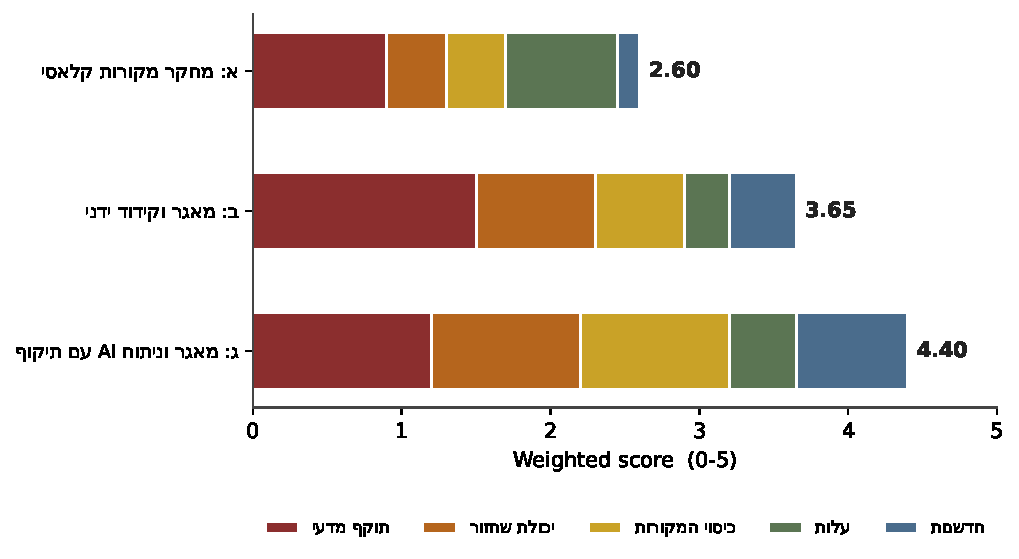
\includegraphics[width=0.85\textwidth]{figures/ch5-decision.pdf}
  \caption{הציון הסופי של כל חלופה, מפורק לתרומת כל קריטריון}
  \label{fig:alt-decision}
\end{figure}

\section{ניתוח רגישות: האם ההחלטה יציבה?}
\label{sec:alt-sensitivity}

ההחלטה תלויה במשקלים, ולכן בדקנו מה קורה כשמשנים אותם. בדקנו בשתי דרכים.

\paragraph{שינוי של קריטריון אחד.} בחרנו לבדוק את התוקף המדעי, משום שזה הקריטריון שבו חלופה ג חלשה מחלופה ב. העלינו את המשקל שלו בהדרגה מ־0 עד 0.9, והקטנו את שאר המשקלים באופן יחסי. כפי שמראה איור~\ref{fig:alt-sensitivity}, חלופה ג נשארת הטובה ביותר עד שמשקל התוקף המדעי מגיע לכ־0.61 – יותר מפי שניים מהמשקל שבחרנו. רק כשהתוקף המדעי שווה יותר מכל שאר הקריטריונים יחד, הקידוד הידני עדיף.

\begin{figure}[htbp]
  \centering
  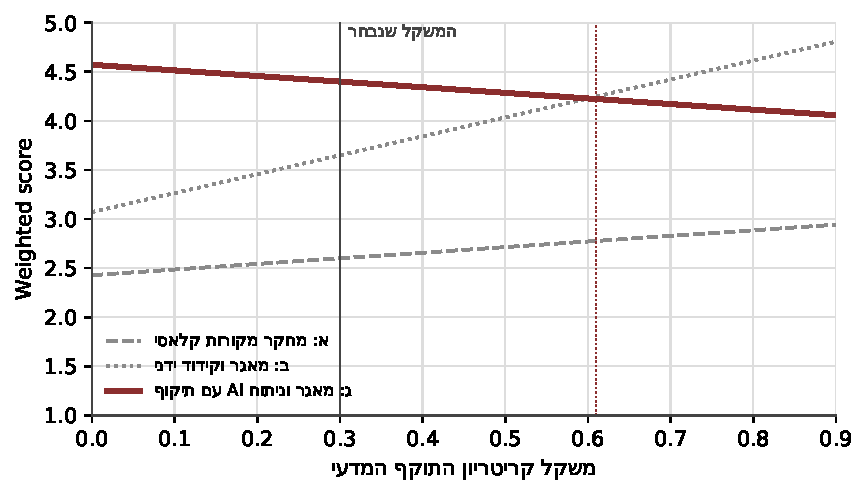
\includegraphics[width=0.85\textwidth]{figures/ch5-sensitivity.pdf}
  \caption{ניתוח רגישות: הציון של כל חלופה כשמשקל התוקף המדעי משתנה}
  \label{fig:alt-sensitivity}
\end{figure}

\paragraph{משקלים אקראיים.} בבדיקה השנייה הגרלנו 10,000 צירופים של משקלים סביב המשקלים שבחרנו, וחישבנו בכל פעם איזו חלופה מנצחת. חלופה ג ניצחה ב־99.6\% מהצירופים, וחלופה ב ב־0.4\% הנותרים. המסקנה היא שההחלטה יציבה: היא אינה תוצאה של בחירה מקרית של משקלים.

\paragraph{מה הבדיקה מלמדת.} מעבר לבחירה עצמה, הניתוח מצביע על נקודת התורפה של החלופה שנבחרה: התוקף המדעי של סיווגי המודל. לכן הארכיטקטורה (סעיף~\ref{sec:alt-architecture}) בנויה סביב תיקוף אנושי, ולכן הטעויות של המודל הן אחד הסיכונים המרכזיים בפרק~\ref{ch:risks}.

\section{ארכיטקטורת המחקר}
\label{sec:alt-architecture}

איור~\ref{fig:alt-architecture} מציג את מסלול הנתונים בחלופה שנבחרה, מהמקורות ועד לתוצאות.

\begin{figure}[htbp]
  \centering
  % figures/ch5-architecture.tex -- research architecture and data flow (chapter 5)
% Colors come from the template; fallbacks are defined here only if missing.
\providecolor{accent}{HTML}{8B2E2E}
\providecolor{accentlight}{HTML}{F4E9E1}
\begin{tikzpicture}[
  node distance=5mm,
  stage/.style={draw=accent, fill=accentlight, rounded corners=2pt,
               minimum width=62mm, minimum height=10mm, align=center, font=\small},
  human/.style={stage, fill=accent, text=white, font=\small\bfseries},
  side/.style={draw=accent, dashed, rounded corners=2pt, align=center,
               font=\footnotesize, minimum width=34mm, inner sep=3pt},
  arrow/.style={-{Stealth[length=2.3mm]}, thick, draw=accent}
]
  \node[stage]  (src)  {\textbf{מקורות}\\ \footnotesize \en{Perseus}, \en{dMGH}, \en{Seshat}};
  \node[stage, below=of src]  (prep) {\textbf{הכנת הקורפוס}\\ \footnotesize חלוקה לקטעים, תיוג מקור, מדינה ותאריך};
  \node[stage, below=of prep] (ai)   {\textbf{סיווג בעזרת מודל שפה}\\ \footnotesize קטגוריות של יחסי כנסייה–מדינה};
  \node[human, below=of ai]  (exp)  {תיקוף בידי מומחה\\ \footnotesize מדגם של 300 קטעים};
  \node[stage, below=of exp]  (db)   {\textbf{מאגר הנתונים}\\ \footnotesize מדינה $\times$ מקטע של 25 שנה};
  \node[stage, below=of db]   (stat) {\textbf{ניתוח סטטיסטי}\\ \footnotesize בדיקת \en{H1}, \en{H2} וניתוח רגישות};
  \node[stage, below=of stat] (out)  {\textbf{תוצאות ופרסום פתוח}\\ \footnotesize קוד, נתונים ומאמר};

  \draw[arrow] (src) -- (prep);
  \draw[arrow] (prep) -- (ai);
  \draw[arrow] (ai) -- (exp);
  \draw[arrow] (exp) -- node[left, font=\footnotesize] {עומד ביעד} (db);
  \draw[arrow] (db) -- (stat);
  \draw[arrow] (stat) -- (out);
  % feedback loop when validation fails
  \draw[arrow, dashed] (exp.west) -- ++(-9mm,0) |- node[pos=0.25, left, font=\footnotesize, align=center] {לא עומד\\ ביעד:\\ תיקון} (ai.west);

  % agent committee beside the AI step (on the right in RTL reading)
  \node[side, right=12mm of ai] (agents) {\textbf{ועדת סוכנים}\\ מסווג\\ מבקר (צוות אדום)\\ בודק נתונים};
  \draw[arrow, dashed] (agents) -- (ai);
  % control variables enter the database directly
  \node[side, right=12mm of db] (ctrl) {\textbf{משתני פיקוח}\\ כלכלה, צבא, אקלים};
  \draw[arrow, dashed] (ctrl) -- (db);
\end{tikzpicture}

  \caption{ארכיטקטורת המחקר: מסלול הנתונים מהמקורות ועד לתוצאות}
  \label{fig:alt-architecture}
\end{figure}

\begin{enumerate}
  \item \textbf{מקורות.} הטקסטים נאספים מ־\en{Perseus} ומ־\en{dMGH}, ששניהם בגישה פתוחה ובפורמט שהמחשב יכול לקרוא (פרק~\ref{ch:market}).
  \item \textbf{הכנת הקורפוס.} כל טקסט מחולק לקטעים קצרים, וכל קטע מקבל תגיות: מקור, מדינה, ומקטע הזמן של 25 שנה שאליו הוא שייך.
  \item \textbf{סיווג בעזרת מודל שפה.} המודל מסווג כל קטע לפי קטגוריות שנגזרות מהמשתנים בטבלה~\ref{tab:variables}: למשל, בישוף בתפקיד ממשלתי, חקיקה דתית מטעם השליט, או סכסוך בין שליט לבישופים.
  \item \textbf{תיקוף בידי מומחה.} מומחה לתקופה מסווג בעצמו מדגם של 300 קטעים, בלי לראות את תשובות המודל, ומשווים בין השניים. אם ההתאמה נמוכה מ־85\%, ההנחיות למודל מתוקנות והסיווג רץ מחדש. זו נקודת הבקרה האנושית של התהליך.
  \item \textbf{מאגר הנתונים.} הסיווגים המאושרים נספרים ומסוכמים לכל מדינה ולכל מקטע זמן, ולצידם נכנסים משתני הפיקוח.
  \item \textbf{ניתוח סטטיסטי.} על המאגר נבדקות ההשערות \en{H1} ו־\en{H2}, עם ניתוח רגישות להגדרות השונות של המדדים.
  \item \textbf{תוצאות ופרסום.} הקוד, הנתונים והקורפוס המתויג מתפרסמים בגישה פתוחה.
\end{enumerate}

\subsection*{ועדת הסוכנים}

שלב הסיווג אינו נעשה בידי מודל אחד, אלא בידי צוות קטן של סוכני \en{AI}, שכל אחד מהם מקבל תפקיד מוגדר בקובץ הנחיות משלו. \textbf{הסוכן המסווג} קורא כל קטע ומסווג אותו. \textbf{הסוכן המבקר}, בתפקיד ״צוות אדום״, מקבל מדגם מהסיווגים ומחפש טעויות, סתירות וסיווגים חשודים. \textbf{הסוכן הבודק} מוודא שהנתונים שלמים ועקביים: שלכל קטע יש מקור ותאריך, ושאין כפילויות. סוכן ראשי מחלק את העבודה ביניהם ומרכז את התשובות. הכלל המנחה הוא הפרדה בין מי שמגלה תקלה לבין מי שמתקן אותה, וההחלטה הסופית נשארת תמיד בידי המומחה האנושי.

\section{החדשנות}
\label{sec:alt-innovation}

המחקר המוצע אינו שכפול של עבודה קיימת. החדשנות שלו נמצאת בארבעה מקומות:

\begin{enumerate}
  \item \textbf{השוואה של שלושה מקרים באותם מדדים.} לפי הסקירה בפרק~\ref{ch:literature}, זו הפעם הראשונה שרומא המערבית, רומא המזרחית והממלכה הפרנקית נבחנות יחד בשיטה כמותית אחת.
  \item \textbf{מדידה של השתלבות, ולא רק של התנצרות.} מחקרים קודמים מדדו כמה אנשים התנצרו; המחקר שלנו מודד \textbf{איך} הכנסייה השתלבה במוסדות המדינה.
  \item \textbf{שילוב של מודל שפה ומומחה.} המחקר מאמץ את המסקנה של מחקרים כמו \en{Ithaca}, שלפיה אדם ומודל יחד עדיפים על כל אחד מהם לבד \cite{assael2022ithaca}, ומיישם אותה בשאלה היסטורית גדולה.
  \item \textbf{תוצרים פתוחים.} המאגר והקורפוס המתויג יעמדו לרשות חוקרים אחרים, ויאפשרו לבדוק גם השערות אחרות על אותה תקופה.
\end{enumerate}
